\chapter{Theory}

\section{Targeted radionuclide therapy}

Today, multiple options are available for treatment of cancerous tissue and diseases, where some of the methods are chemotherapy, surgery, immunotherapy, external beam-therapy, brachytherapy and targeted radionuclide therapy \textcolor{red}{citation}. The latter three treatment types utilizes ionizing particles to induce damage in the DNA of cancerous cells, so that they undergo apoptosis. In external beam therapy, photons, electrons or hadrons are accelerated and focused towards a tumor externally, and in bracytherapy an unsealed radioactive source (usually a wire or pellet containing for instance a $\beta^-$-emitter), is placed in proximity to tumor. Targeted radionuclide therapy is an emerging alternative to the traditional treatment options, inwhich can deliver a cytotoxic level of dose to the site of disease (all from handbook of nuclear chemistry, "Targeted radionuclide therapy - introduction", p. 2180). It offers a patient-specific treatment dependent on choice of radiopharmaceutical which targets a type of tumor or cell. A radiopharmaceutical consists of a radionuclide and a cell-targeting molecule called a tracer.  Meanwhile brachytherapy and targeted radionuclide therapy are limited by the cancer location and the existence of metastasis, along with required knownledge of the tumor to maximice the dose over the tumor and minimizing the dose to healthy tissue (Handbook of nuclear chemistry, p. 2180), targeted radionuclide therapy utilizes the biochemical pathways in the body, thus with an appropriate tracer, targeted tissue with an high uptake of the radiopharmaceutical will receive a high dose, and healthy tissue can be spared (Yeong2014).\\ 

\noindent 



\noindent    \textcolor{blue}{Whenever something is cited like (3), it means citation 3 in special curriculum}
Special curriculum p. 4: many requirements before a radiopharmaceutical can be used clinically, there are physical properties concerning the radionuclide, such as physical half-life, decay-mode and decay product, radiation energy and in-tissue range, and biological properties concerning the tracer such as tissue targeting, biological half-life, retention in tumor and the uptake in healthy tissue (3). Thus, the radiopharmaceutical requires two components in which complement each other to deposit the dose in the cancerous tissue. For the tracer, a rapid blood clearance and transport (6, p. 145) and high uptake and retention in the tumor (9. p. 2)    (special curriculum p. 4) are important characteristics. It can target the desired cells by for instance a specific receptor, enzyme, membrane, transporters or antigens (6, p. 145). Radiometals are also used, which consists of a bifunctional chelator, which is a molecule containing molecules which can donate a lone pair of electrons, like nitrogen, oxygen or sulfur. If the radiometal has an oxidation state of $3^+$, it will be tighlty bound by the chelator, and can transported to the tumor (special curriculum p. 4-5). \\

In nuclear medicine, the effective half-life of the radiopharmaceutical is important as it takes both the physical half-life and the time it takes for the radiopharmaceutical to be cleared or excreted from the body (3). The choice of radionuclide should match the uptake rate and the retention, to avoid radioactive waste handling and dose to healthy tissue (3). Therapautic radionucldies typically have half-lives  in order of a few hours to several days (9, p. 1) (special curriculum p. 4).\\

Knowledge about the decay products are also important, if unstable, how it the dose distributed, and how long range, half life, blabla, and if unstable, is the daughter contributing to a cytotoxic effect, or taking part of the natural stuff in the body. \\

The radiation range in tissue is important. Different decay-modes result in particle with different ranges in tissue, Dependent on the size of tumor and critical target surrounding it, different emitters are used. However to reduce the dose to healthy tissue, specific short range high LET particles such as auger electrons, alpha-particles and beta-particles are in general desired. Figure \ref{fig:cell_dimension} shows the ranges of auger electrons, alpha-particles and $\beta^-$-particles on a cellular scale. In a medium, there are positively charged nuclei and negatively charged electrons. We differ between neutral particles like neutrons and photons, and charged particles like electrons or protons, alpha-particles, and other heavy charged particles. Charged particles have a short range in comparison to neutral particles, as the Coloumforce forces the particle to interact continously along the path, either either by scattering inelastically with the atomic electrons, or scattering elastically via the nuclei. Inelastic collisions is the dominant process, where the atomic electrons are either excited or ionized. The maximum energy transfer (under the assumptions particle moves rapidly, collision is head-on, energy transferred is large compared with the binding energy, energy is free and at rest, and collision is elastic )

\begin{equation}
    Q_\text{max}=\frac{4mME}{m+M}
\end{equation}
where E is initial kinetic energy of particle, m is electron mass and M is incident particle mass \footnote{https://ocw.mit.edu/courses/nuclear-engineering/22-55j-principles-of-radiation-interactions-fall-2004/lecture-notes/energy_depos_hcp.pdf}. If the now free electron had sufficient energy transferred from the incoming particle (called a $\delta$-electron), this electron can further ionize along the particle track. Elastic scattering is the less dominant process, where the energy loss is small, as long as the nuclei in the medium are larger than the incoming particle (Techniques for Nuclear and Particle Physics Experiments, William R. Leo, p. 21). The energy loss of heavy charged particles are described by an equation called Bethe-Block, where the energy loss at high energies is small since very little energy is transferred per collision with atomic electrons (due to the large mass).  The stopping power is proportional to

\begin{equation}
    \frac{dE}{dx}\propto \frac{z^2}{\beta^2}\frac{Z}{A} \rho,
\end{equation}

the charge of the particle z squared, the velocity squared ($\beta=v/c$), and the atomic and mass number of the material and the density (Techniques for Nuclear and Particle physics experiments, p.  24). So alpha-particles are stopped rather quickly and have a high linear energy transfer. 
When the particle reaches low velocity, the particle interacts at a much higher rate in a very specific peak called the Bragg peak. Can be seen on figure \ref{fig:particle_interaction}, for the proton. As we can see, the energy deposited behind the tumor is almost zero, along with the energy deposition in front of the tumor is low which is something which can utilized in radiation therapy. However, since the Bragg peak is so narrow, a broadening of the beam might be necessary, which is to send out a beam of multiple energies, so that it is spread out. The dose in front of the tissue gets larger, but the dose behind is still zero. The electrons/positrons interacts differently, since the mass is equal to the atomic electrons, the energy transfer can be upto half of its mass, and it scatters like crazy. Electrons can experience energy loss either from collisions like heavy charged particles, or via the electromagnetic radiation that arises when electrons are loosing energy (bremsstrahlung). However, for energies up to a few MeV, the collision energy loss dominates (Techniques for Nuclear and Particle Physics Experiments, William R. Leo, p. 37). On figure \ref{fig:particle_interaction}, we see that  the electrons and proton interacts differently, there is no clear peak, and the incoming electrons immediately interacts with the medium, lose energy fast and the secondary electrons interacts after and slowly decreasing. At 22 MeV, bremsstrahlung stopping power is also evident, so we see an exponential tale which ....? \\

Neutral particles photons and neutrons interacts differently, as they do not lose energy from the coulomb force, the energy is not degraded as the cp, and the beam is attenuated as  afunction thickness x (Techniques for Nuclear and Particle Physics Experiments, William R.Leo, p.  53)

\begin{equation}
    I(x)=I_0 e^{-\mu x}
\end{equation}


\begin{figure}
    \centering
    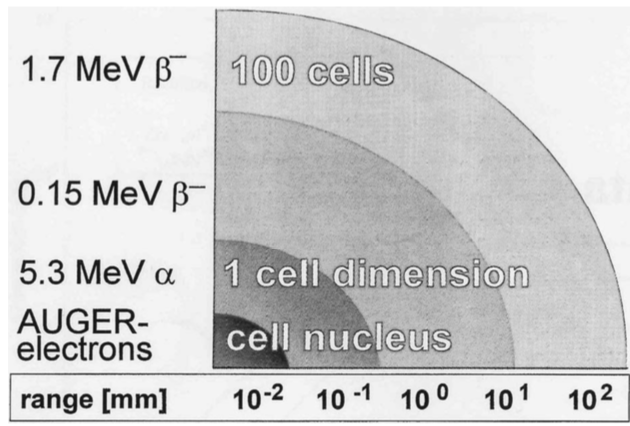
\includegraphics{Theory/cell_dimension.png}
    \caption{The figure illustrates the ranges of different particles on the scale of cells. Auger electrons does not exceed the cellular nucleus and alpha-particles does not exceed more than ca. 1 cell dimension which allows for very specific targeting of cells. Low energetic $\beta^-$ emitters have ranges of ca. 1 mm. Picture is from (S M Qaim, R Capote, and F Tarkanyi.  Nuclear Data for the Production of Therapeutic Ra-dionuclides.Trs 473, (473):395, 20), p. 2. }
    \label{fig:cell_dimension}
\end{figure}


\begin{figure}
    \centering
    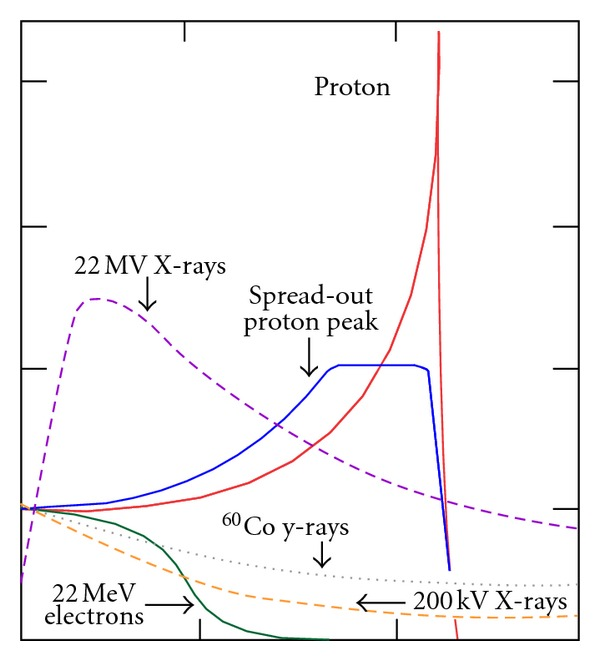
\includegraphics[width=0.6\textwidth]{Theory/Bragg-peak-and-Spread-Out-Bragg-Peak-SOBP-for-a-proton-beam-in-comparison-with-photon.jpg}
    \caption{Medium depth along x-axis, energy deposition in tissue (or dose?) on y-axis. Find citation in special curriculum. }
    \label{fig:particle_interaction}
\end{figure}


The charged particles interacts via inelastic and elastic collisions with the atomic electrons, and the maximum energy transfer (under the assumptions particle moves rapidly, collision is head-on, energy transferred is large compared with the binding energy, energy is free and at rest, and collision is elastic )

\begin{equation}
    Q_\text{max}=\frac{4mME}{m+M}
\end{equation}

where E is initial kinetic energy of particle, m is electron mass and M is incident particle mass \footnote{https://ocw.mit.edu/courses/nuclear-engineering/22-55j-principles-of-radiation-interactions-fall-2004/lecture-notes/energy_depos_hcp.pdf}.  

Thus, electrons can lose up to half of its energy in one elastic collision while heavy charged particles, the collision loss is very small. The main loss of heavy charged particles is described in the equation Bethe-Block, which describes the stopping power heavy charged particles. Right before the particle stops, the majority of the energy is deposited in the Bragg peak, which is very specific, and is advantageous in external radiation therapy. The stopping power is proportional to 

\begin{equation}
    \frac{dE}{dx}\propto \frac{z^2}{\beta^2}\frac{Z}{A} \rho,
\end{equation}

the charge of the particle z squared, the velocity squared ($\beta=v/c$), and the atomic and mass number of the material and the density (Techniques for Nuclear and Particle physics experiments, p.  24). So alpha-particles are stopped rather quickly and have a high linear energy transfer. 




%in order to deposit the therapautic dose in the cancerous tissue, and avoid dose to healthy tissue. 
%When it comes to choice of radionuclide, there are different features that are important. 


\noindent
Along with the ability to use radionuclides in therapy, radionuclides can also be used for diagnostic purposes with imaging, either with positron emitters (positron emission tomography) inwhich annihilates with atomic electrons close to the cite of decay, and sends out two 511 keV photons, or emission of a strongly fed gamma-decay energy which is detected (single photon emission tomography). The combination of a diagnostic and a therapautic agent with similar properties so that the biochemical uptake in the body is a new approach in which can give information of how the uptake is distributed in the body, and can image the state of decease after therapies (The beginning and development of the theranostic approach in nuclear medicine.... 86/90Y). This is called theranostics.. 

\textcolor{red}{Write more detailed about what it is..}

In treatment of diseases related to the use of radionuclides, there are multiple properties that plays an important role, such as physical features like half-life, decay-mode, decay-products, radiation energy and linear energy transfer, and biochemical features like in tissue range, tissue targeting of tracer, uptake and retention in desired tissue, biological half-life and toxicity of radionuclide and decay-product (Yeong, therapautic radionuclides in nuclear medicine). In addition, the availability, cost and quality is important, and that the production routes gives high isotopic purity of the product, along with high yield (Qaim, Nuclear Data for production of medical application of radionuclides: present status and future needs). 


Here write about the varios small things. Isotopic purity, half-life, 


\subsection*{\centering{\small{Particle interaction in matter}}}
\noindent 

\textcolor{red}{equation $$Q_\text{max}=\frac{4mM E}{m+M}$$ can be from billiard physics, or inelastic collision physics. Also, bethe-block is proportional to 
\begin{equation}
    -\frac{dE}{dx}=2\pi N_a r_e^2 m_e c^2\rho \frac{Z}{A}\frac{z^2}{\beta^2}\Big[\ln \Big( \frac{2m_e \gamma^2 v^2 Q_\text{max}}{I^2} \Big)-2\beta^2 -\delta - 2 \frac{C}{Z}\Big]
\end{equation}
where $r_e$ is electron radius, $m_e$ electron mass, $N_a$ avogadro, I mean excitation potential, Z \& A atomic number and mass numer of absorbing material, $\rho$ density of absorbing material, z charge of incident particle, $\beta=v/c$, $\gamma=1/\sqrt{1-\beta^2}= 1/\sqrt{1-v^2/c^2}$, $\delta$ density correction, C shell correction, $W_\text{max}$ is max energy transfer per collision. In general, $$\frac{dE}{dx}\propto \rho,\frac{z^2}{\beta^2},\frac{Z}{A}$$ and logarithmic stuff which i dont know... so alpha particles are stopped quicker than protons if they have the same energy (Techniques for Nuclear and Particle physics experiments, p. 24). }
Particles interact differently in a given medium. Figure \ref{fig:particle_interaction} shows how various particles interacts in a medium where the depth is on the x-axis and dose is on the y-axis. In a medium, there are positively charged nuclei and negatively charged electrons. We differ between neutral particles like neutrons and photons, and charged particles like electrons or protons, alpha-particles, and other heavy charged particles. Charged particles have a short range in comparison to neutral particles, as the Coloumforce forces the particle to interact continously along the path, either either by scattering inelastically with the atomic electrons, or scattering elastically via the nuclei. Inelastic collisions is the dominant process, where the atomic electrons are either excited or ionized. If the now free electron had sufficient energy transferred from the incoming particle (called a $\delta$-electron), this electron can further ionize along the particle track. Elastic scattering is the less dominant process, where the energy loss is small, as long as the nuclei in the medium are larger than the incoming particle (Techniques for Nuclear and Particle Physics Experiments, William R. Leo, p. 21). The energy loss of heavy charged particles are described by an equation called Bethe-Block, where the energy loss at high energies is small since very little energy is transferred per collision with atomic electrons (due to the large mass). However, when the particle reaches low velocity, the particle interacts at a much higher rate in a very specific peak called the Bragg peak. Can be seen on figure \ref{fig:particle_interaction}, for the proton. As we can see, the energy deposited behind the tumor is zero, along with the energy deposition in front of the tumor is low which is something which can utilized in radiation therapy. However, since the Bragg peak is so narrow, a broadening of the beam might be necessary, which is to send out a beam of multiple energies, so that it is spread out. The dose in front of the tissue gets larger, but the dose behind is still zero. The electrons/positrons interacts differently, since the mass is equal to the atomic electrons, the energy transfer can be upto half of its mass, and it scatters like crazy. Electrons can experience energy loss either from collisions like heavy charged particles, or via the electromagnetic radiation that arises when electrons are loosing energy (bremsstrahlung). However, for energies up to a few MeV, the collision energy loss dominates (Techniques for Nuclear and Particle Physics Experiments, William R. Leo, p. 37). On figure \ref{fig:particle_interaction}, we see that  the electrons and proton interacts differently, there is no clear peak, and the incoming electrons immediately interacts with the medium, lose energy fast and the secondary electrons interacts after and slowly decreasing. At 22 MeV, bremsstrahlung stopping power is also evident, so we see an exponential tale which ....? \\

Photons interacts differently than charged particles. As they are neutral, they do not interact via inelastic collisions, but interacts via three different processes called photoelectric effect, compton scattering and pair production. Thus the energy is not degraded, and the beam can only be attenated as a function of thickness x (Techniques for Nuclear and Particle Physics Experiments, William R. Leo, p. 53)
\begin{equation} \label{eq:intensity_photons}
    I(x) = I_0 e^{-\mu x}
\end{equation}

where $\mu$ is the attenuation coefficient. Photons can be gamma-rays or X-rays, where gamma-rays are produced in de-excitation of nuclei, and have ranges 0.1-10 MeV (Krane, p. 327), and X-rays can be either be produced in de-exciation of atomic electrons (where the energies are typically quite low), or be produced by de-accelerating fast electrons in an x-ray tube, for instance by hitting a material like tungsten, where the energy is high. As we can see on figure \ref{fig:particle_interaction}, the X-rays are produced in an x-ray tube (MV and kV is the voltage of the X-ray tube), and we can see that the 22 MV X-rays have a build-up effect, where ionized atomic electrons participates in increasing the dose, while the much lower 200 kV X-rays does only de-crease. The gamma-rays from $^{60}$Co behaves similarly to the 200 kV X-rays, but are slighlt higher in energy deposition as the energy in general are slighly higher than 200 keV. The tale is exponential as we can see in eq. \ref{eq:intensity_photons}, and is in fact a problem in radiation therapy as the dose to healthy tissue behind the tumor is quite high. 

Photoelectric effect dominates at lower energies, and happens when a photon (energy) is completely absorbed an atomic electron. In gamma-ray spectroscopy, this process is desired as the gamma-rays from nuclei is specific, and we can identify the nuclei on a spectrum. Probability of photoelectric effect is \begin{equation}
    \tau \propto \frac{Z^n}{E_\gamma^{3.5}}, \quad \text{n= 4 or 5}
\end{equation}
where Z is the atomic number of material ((Techniques for Nuclear and Particle Physics Experiments, William R. Leo, p. 55). 

In compton scattering, the photon has higher energy and can transfer parts of the energy to an atomic electron, be deflected and ionize further. The deflecting angle is dependent on energy, and the angle $\theta\in (0^\circ, 180^\circ)$ (Techniques for Nuclear and Particle Physics Experiments, William R. Leo, p. 55-56). Compton scattering thus gives photons in a spectrum of different energies. This process is not desired in gamma-ray spectroscopy, and contributes to noise in a Compton region. This process is however desired in external radiation therapy, as the process gives rise to high energetic secondary electrons, and photons in which ionize further. The probability of interaction is 
\begin{equation}
    \sigma \propto Z
\end{equation}

Pair production demands a photon energy to be equal or higher than two electron rest  masses, as the photon is converted to an electron/positron pair (1.022 MeV=2$m_0c^2$) (Techniques for Nuclear and Particle Physics Experiments, William R. Leo, p. 57). Probability of interaction is \begin{equation}
    \kappa\propto Z^2
\end{equation}

Finally neutrons interacts with the strong force with nuclei, and can be via absorption, or elastic or inelastic scattering. The interaction probability is dependent on energy, will not describe more. (Techniques for Nuclear and Particle Physics Experiments, William R. Leo, p. 64). 

Whenever a charged particle like an electron or hadron enters a medium, the Coloumbforce will affect the charged particle and cause interactions with the atomic elecrtons. Neutral particles like photons and neutrons are not affected by the Coulomb force, thus interacts rarely. On figure ..., the 22 MV X-rays first has a build-up effect, where the initial photons induce ionzations and secondary electrons, which contributes to further ionization, and increases the dose. After, the dose decreases exponentially. 
The build-up effect for high-energetic photons which are only used in external beam therapy enables an energydependent maximum dose in tissue as a function of depth. However, the exponential tale gives dose to the healthy tissue behind. The gamma-rays in nuclei are not that energetic, and the lack of specificity does not make gamma-rays a suitable decay chain for therapeutic agents. Neutral particles interacts via absorption or   \\



\begin{figure}
    \centering
    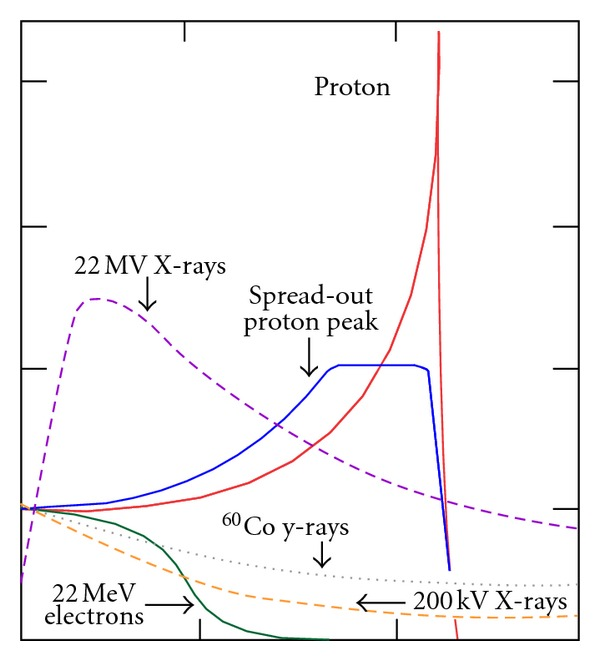
\includegraphics[width=0.6\textwidth]{Theory/Bragg-peak-and-Spread-Out-Bragg-Peak-SOBP-for-a-proton-beam-in-comparison-with-photon.jpg}
    \caption{Medium depth along x-axis, energy deposition in tissue (or dose?) on y-axis. Find citation in special curriculum. }
    \label{fig:particle_interaction}
\end{figure}




\textcolor{red}{
A way to work around this is to rotate the beam around the patient which relieves the healthy tissue and give maximal dose to tumor. Also a note, gamma-rays are typically in the energy region from 0-3000 keV, thus does not give sufficiently high dose for treating a tumor. 

X-rays from an accelerator is produced by acceleration of electrons which hits a material like for instance wolfram or tungsten. The X-rays have energies ranging from zero to the max electron energy, and hence the X-ray energy is in MV instead of MeV. 
Why we are not using gamma-rays in treatment; range is too long, ionization are not frequent enough, and energy is too low?}


\subsection*{\centering{\small{The biological effect of ionizing radiation and linear energy transfer}}}
\textcolor{red}{in general in this paragraph refer to the radiation biology book.. }
Ionizing radiation are particles with sufficient energy to cause ionizations along the particle track, thus separating an atom and one or more electrons \textcolor{red}{citation, maybe the bio-book?}. The free electron(s) can ionize further, and the positive ion can cause undesired reactions \textcolor{red}{find a citation}. DNA is a large molecule with two strands bound in a double helix structure. Each strand is composed of sugar and phosphate groups, and nitrogenous bases which bind the two strands. These bases are called adenin \& guanin and cytosine \& thyamin (always bound pairwise), and are bound through weak hydrogen bonds which are exposed to strand breaks. The cell is equipped with an impressive repair mechanism, and  unless both DNA strands are damaged, which is called a double stranded break (DSB), most damages are repaired \textcolor{red}{cite}. Radiation damages in the DNA can be caused directly by the ionizing particle, or indirectly via free radicals which are subject to other ionizations.  Since the body contains large amounts of water, ionization of water molecules giving for instance H$^\bullet$ or OH$^\bullet$ are important damaging factors. Damages induced in the DNA can be lethal to the cell and either cause apoptosis or mutation in which can be a cause of cancer. In therapy, the goal is to make the cancerous cells to undergo apoptosis, and choosing a particle which has a high probability of inducing damage will induce multiple double stranded breaks, if passing nearby. \\

\noindent 
Linear energy transfer (LET) describes the energy absorbed by the medium, and is defined as the  average energy (typically measured in keV) deposited per unit length (typically measured in $\mu$m) of the density material (book, p. 101):

\begin{equation}
    \text{LET} = \frac{dE}{dx}
\end{equation}

\noindent 
LET thus describes the general frequency in which a particle will deposit energy along the particle track. A particle with a high LET-value will interact more frequently over a shorter distance than a low LET-particle. In targeted radionuclide therapy, it is important that the range of the particle is short-range so that the healthy tissue is spared, and that the dose to the cancerous tumor is large. For therapy, medical isotopes which emit radiation with high LET such as $\alpha$, $\beta$ and auger-electrons are desired since the ionization rate is high and the distance traversed is low (Yeong, therapautic radionuclides in nuclear medicine). Gamma-radiation is not a desired process in therapy as photons does not degrade in energy, thus can have a long range unless attentuated. 
Figure \textcolor{red}{...} shows how alpha, beta and auger electrons interacts on the scale of DNA. \\


\subsection*{\centering{\small{Decay modes}}}

Different decay modes have different ranges in the tissue. Dependent on the size of tumor, and critical tissue surrounding it, different emitters are used. However to reduce dose to healthy tissue, specific short range high LET particles are in general desired. Figure \ref{fig:cell_dimension} shows the ranges of auger electrons, alpha-particles and $\beta^-$- particles on a cellular scale. The binding energy holds the nucleus together, and for unstable nuclei, the binding energy is so low that particles can be emitted to gain stability, lowering the binding energy. Beta and alpha decay changes the element, and the decay product is commonly in an excited state. Therefor gamma-decay commonly occurs after, and in gamma-ray spectroscopy, it is the gamma-rays of the de-exicitation of the daughter which is detected. Knowledge about the energy and intensity of the radiation is very important. It is unrare that just one single process happens during a decay, and dependent on what the desired process is, there is a beta or alpha particle or gamma-rays, X-rays or auger electrons caused from electron capture or internal conversion. The ranges can be different. \\ 

\noindent
Beta-decay happens whenever there is an overweight in number of protons or neutrons. For an overweight of neutrons, $\beta^-$-decay occurs, by transforming a neutron into a proton, a $\beta^-$-particle and an antineutrino

\begin{equation}
    n \rightarrow p + e^- + \overline{{\nu_e}}
\end{equation}

\noindent
For an overweight in protons, $\beta^+$ decay occurs, by transforming a proton into a neutron, a $\beta^+$-particle and a neutrino

\begin{equation}
    p \rightarrow n + e^+ + {\nu_e}
\end{equation}

$\beta^+$-particles are typically used in diagnostic imaging in PET (positron emission tomography). 
\noindent Since neutron mass is higher than the proton mass (mass difference 1.022 MeV/$c^2$), there is ad attidional threshold energy needed to induce the reaction. If the energy is not high enough, electron capture dominates, which takes in an atomic electron (typically from K-shell), and with a proton in the nucleus, transformning to a neutron and a neutrino:
\begin{equation}
    p + e^- \rightarrow n + \nu_e 
\end{equation}

Since beta-rays are not monoenergetic, the energy is distruted between three particles and gives a spectrum of different possible energies. $\beta^-$-emitters used in therapy is stopped rather quickly in tissue due to negative charge and low mass (as mentioned in the above section, energy transfer can be up to half of its mass. ), 

Alpha-particles are $^{4}$He-nuclei, consisting of two protons and two neutrons. It is emitted from heavy nuclei. Since the nuclear force is short range (1fm ?), and heavy nuclei tend to be in the limit between electromagnetic and nuclear force, an alpha particles (which carries large binding energy) lowers the binding energy sufficiently so that the nucleus is more stable. The binding energy of an alpha particle is very high (28.3 MeV) which is why an alpha-particle is emitted to lower binding energy. 

Gamma-decay is emission of photons following de-excitation of the nucleus, as de-excitation from one state to another. It is specific for the nucleus, and is thus called the fingerprint of the nucleus, because we can observe it for instance in a gamma-ray spectrum. Gamma-decay commonly occurs after beta or alpha decay, or can happen if there is an isomer, then the decay mode is called isomer transition. However, gamma-rays are not well suited in therapy them selves (however for imaging in SPECT more relevant). But nuclei that emit electrons following gamma-decay are more relevant. Internal conversion is a process where the gamma-ray interacts electromagnetically with atomic electrons, and the electron is emitted instead of the photon. This electron is called an conversion electron and has energy in the order of the gamma ray (minus atomic binding energy). In order to fill the atomic shells, a cascade of X-rays and auger electrons are emitted (auger electrons have energies in order of X-rays). 


\begin{figure}
    \centering
    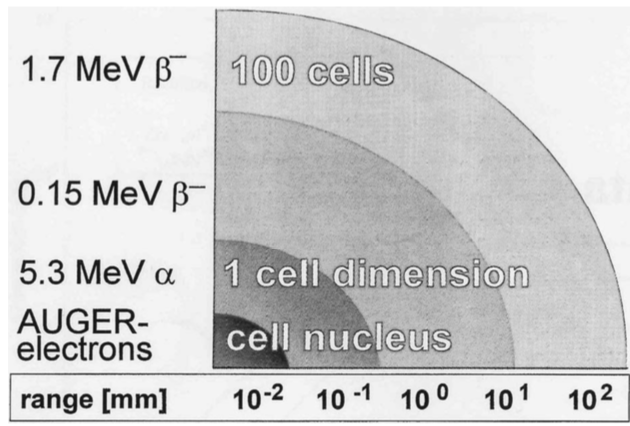
\includegraphics{Theory/cell_dimension.png}
    \caption{The figure illustrates the ranges of different particles on the scale of cells. Auger electrons does not exceed the cellular nucleus and alpha-particles does not exceed more than ca. 1 cell dimension which allows for very specific targeting of cells. Low energetic $\beta^-$ emitters have ranges of ca. 1 mm. Picture is from (S M Qaim, R Capote, and F Tarkanyi.  Nuclear Data for the Production of Therapeutic Ra-dionuclides.Trs 473, (473):395, 20), p. 2. }
    \label{fig:cell_dimension}
\end{figure}



\subsection{$\mathbf{^{193m}}$Pt as a potential therapautic agent}
$^{193m}$Pt ($t_{1/2}$=4.33 days) is an auger-emitting isomer which decays by isomeric transition (100\%) to the long-lived $^{193g}$Pt groundstate ($t_{1/2}$=50 years). Radionuclides produced from deuterons on natural iridium such as $^{191}$Pt, $^{193m}$Pt, $^{192}$Ir and $^{194}$Ir are believed to have potential in medicine, like chemotherapy, brachytherapy, radioimmunotherapy and imaging (Tarkanyi et.al 2006). Platinum radionuclides are of special interest, as platinum is the main element in chemotherapautic agents such as cisplatin, which is a drug which is used clinically in treatment of testicular and ovarian cancer mainly, but also to treat esophagus, head and neck and bladder cancer\footnote{https://www.sciencedirect.com/science/article/pii/S0969804399000822?casa_token=ZLJ8YPQzGZMAAAAA:264QzKWpH8Kv6iHotiGMeoHTk8jKqmnoDgf709SrAD8BUWVwbRXriZbHgkYO_tHg-2qyX3Hvt9E}. Cisplatin  (cis-dichlorodiammine platinum(II)) is an inorganic molecule which contains one stable platinum atom surrounded by two clorine atoms and two ammonia molecules (NH$_3$). The cisplatin-molecule enters the cell nucleus, and binds to the DNA, example-wise shown in figure \ref{fig:cisplatin_DNA}, where the clorine-atoms are de-attached and the platinum-atom binds through covalent bonds to the DNA base guanine (and in some cases adenine, \textcolor{red}{is that correct?}), and breaks the bonds between the DNA nitrogeneous bases. Cisplatin thus targets the DNA. One of the major challenges with cisplatin is the chemical toxicity, but when auger-emitters such as $^{193m}$Pt or $^{195m}$Pt replace the stable platinum atom, the local auger-damage effect increases the chemical damage of cisplatin, suggesting that a smaller amount of the drug is required, and chemical toxicity can be avoided \footnote{http://citeseerx.ist.psu.edu/viewdoc/download?doi=10.1.1.987.2577&rep=rep1&type=pdf#page=506, p. 493}. 

By replacing either of the stable nitrogen atoms with the PET-radionuclide $^{13}$N ($t_{1/2}$=9.965 minutes), or by a radionuclide platinum, where $^{191}$Pt ($t_{1/2}$=2.83 days, decay by electron capture (100\%) to $^{191}$Ir (stable)) , $^{193m}$Pt and $^{195m}$Pt ($t_{1/2}$=4.010 days, decay by isomer transition (100\%) to $^{195g}$Pt (stable)) is of special interest, cisplatin can be used for imaging or therapy\footnote{https://www.sciencedirect.com/science/article/pii/S0969804399000822?casa_token=ZLJ8YPQzGZMAAAAA:264QzKWpH8Kv6iHotiGMeoHTk8jKqmnoDgf709SrAD8BUWVwbRXriZbHgkYO_tHg-2qyX3Hvt9E}, but therapy is most common. \\ 

\noindent 
As $^{191}$Pt is electron-capture emitter, can be used in imaging, with for instance 129.4 keV (38.0\%) or 172.19 keV (43.2\%). Combining $^{191}$Pt with a therapautic agent might be possible for theranostic pair with either $^{193m}$Pt or $^{195m}$Pt? Can be combined with therapy as it releases auger electrons? \\

\noindent
Decay mode: For $^{193}$Pt, there are three states, the isomer state at 149.8 keV, with nuclear spin $13/2^+$ (4.33 d), a state at 14.3 keV with nuclear spin $5/2^-$ (2.52 ns), a state at 1.6 keV with nuclear spin $3/2^-$ (9.7 ns) and the ground state at 0.0 keV with nuclear spin $1/2^-$ (50 y)\footenote{https://www.nndc.bnl.gov/nudat2/getdecayscheme.jsp?nucleus=193PT&dsid=193pt%20it%20decay%20(4.33%20d)&unc=nds
}\footenote{Shirley, V.S. Nuclear data sheets for A=193. Nucl. Data Sheets. 32, 593-679, 1981}. \textcolor{red}{here write about gamma-decay and that the probability for M6 or whatever transition is improbable}. The populated isomer states decays from 149.8 keV to 14.3 keV releasing a 135.50 keV photon (0.1145475\%), from 14.3 keV to 1.6 keV releasing a 12.634 keV photon (0.70\%), and from 1.6 keV to the ground state releasing a 1.642 keV photon (0.0321). The photon abundance is thus low, and this isomer is not well suited for imaging. Due to the low intensity of the gamma-rays, it might be difficult to detect. There are X-rays too, but they overlap with other nuclei. Since the gamma-rays are weak, the IC probabilities are 99.89\%, 99.33\% and 99.99\% for each state respectively, calculated by subtracting 100 - gamma-intensity \footnote{http://citeseerx.ist.psu.edu/viewdoc/download?doi=10.1.1.987.2577&rep=rep1&type=pdf#page=506, p. 496}. This also indicates that the phondon abundance is very low, as well  high very high prob of low E electrons :D 

In all decays, there are certain quantities in which needs to be conserved; angular momentum ($\ell$) and parity (maybe $\ell$ should be written as L instead??). Krane says that a multipole of order $\ell$ transfers angular momentum $\ell\hbar$ per photon (Krane, p. 333). A nuclear state has a definite angular momentum (angular momentum and spin) and parity, and if a gamma-transition is to happen between two states, the photon must connect the two states by conserving angular momentum and parity. In order for the quantity $\ell$ to be conserved, the angular momentum can be integer values between
\begin{equation}
|I_i-I_f| \leq \ell \leq I_i + I_f
\end{equation}
For the decay of $^{193m}$Pt (E level=149.8 keV) to the excited state (E level=14.3 keV), the spin and parity change is from $13/2^+$ to $5/2^-$, so $\ell=4,5,6,7,8,9$. The parity decides the wether the radiation is electric multipole or magnetic multipole (equations from Krane p. 331), 

\begin{equation}
    \pi(ML) = (-1)^{\ell+1}, \quad \pi(EL)=(-1)^{\ell}
\end{equation}
 
The electric decays have even parity when $\ell$=even, and magnetic has even when $\ell$ is odd. If parity is unchanged in the reaction ($\Delta \pi=$no), the electric multipoles are even and magnetic multipoles are odd. If the parity does change ($\Delta\pi=$yes), there would be odd electric and even magnetic multipoles. Hence the possible transition from $13/2^+$ to $5/2^-$ are whenever $\Delta \pi=$yes and $\ell=4,5,6,7,8,9$, which gives possible M4, E5, M6, E7, M8 or E9. 

In general, the lowest possible multipole dominates, and the emisssion of multipole of one order higher (L+1 than L), is reduced by a factor ca $10^{-5}$ (Krane p. 335, important!!). Thus, a multipole of order 4 or 5 has a low probability of occuring and thus the isomer has a long half life.  
In comparison to decay from isomer state, decay from $5/2^-$ to $3/2^-$ gives possible radiation, $\ell=1,2,3,4$, with no parity change, and $\Delta \pi=$no, gives possible M1, E2, M3, E4, and from $3/2^-$ to $1/2^-$ gives $\ell=1,2,3,4$, which also gives M1,E2, M3, E4. 

Half life: the decay rate constant is the sum of the decay rates of all the populates states  transitions, $\lambda=\lambda_{13/2^+} + \lambda_{5/2^-}+ ...$. 







\subsubsection{Gamma-decay and isomeric transition}
Gamma-decay is the lowering of the excitation energy by the release of a photon, with an energy $\Delta$E equal to the energydifference in the two states. The typical half lives of gamma-emission are less than $10^{-9}$ seconds, however, longer lived states of a nucleus which is not the ground state is called an isomer, and the gamma-decay of an isomer state is called isomeric transition (Krane, p. 175). Whenever gamma-decay is possible, another process called internal conversion is competing. It is an electromagnetic process, where the nucleus interacts electromagnetically with the atomic electrons, and an electron is emitted instead of the photon (Krane, chapter 10, p. 341). The kinetic energy of the emitted electron is the transition energy minus the electron binding energy

\begin{equation}
    T_e = \Delta E - B
\end{equation}

where B is a positive number (even though bound states are negative??). The electron is called a conversion electron, and this electron is high in energy and mathces the gamma-energy. 
The electron binding energy varies with the atomic orbital (Krane), and the electrons emitted following internal conversion are in a spectrum of different discrete energies. The transition energy must be higher than the electron binding energy, and as a consequence, the electron is labelled with the shell that it was emitted from. (remember, n=1=K, n=2=L, n=3=M, n=4=N) \\ 

In the case of the decay of $^{193m}$Pt, internal conversion is highly favoured instead of gamma-decay (the intensity of the gammas are very weak). The total decay probability is the summed decay probability for gamma-decay and internal conversion
\begin{equation}
\lambda = \lambda_\gamma + \lambda_{IC}    
\end{equation}

and the internal conversion coefficient $\alpha$ can be defined as
\begin{equation}
    \alpha = \frac{\lambda_{IC}}{\lambda_\gamma}
\end{equation}

High values of $\alpha$ indicates high probability of internal conversion, relative to probability of gamma-emisson, but the coefficient diverges towards infinity when $\lambda_\gamma$ reaches towards zero, which for instance is when the gamma-transition is zero. In general, the coefficient increases as $Z^3$, which will give a much greater coefficient for heavy nuclei than for lighter nuclei. In addition the coefficient decreases rapidly (ca. $E^{-2.5}$) with increasing transition energy. The multipole order also affects the coefficient, where a higher multipole order indicates a higher value. For higher atomic shells than the K shell (n=1), the coefficient decreases like $n^{-3}$ (Krane, chapter 10, p. 346). \\

\noindent 
In therapy, the most important process is the process which occurs after the release of the conversion electron. There is a vacancy in the shell where the conversion electron was emitted, and an electron from a higher shell drops down to this energylevel, with the release of an X-ray with an energy equal to the difference between the energy state of the two shells, $\Delta E$.\textcolor{red}{ If the transition is an electron from an L shell drops to K shell, and an electron from the L shell is ejected, the processes is called a KLL transition, and the energy of the auger electron is $E_{auger}=E_K - E_{LL}$ (Prasad A. Naik, in Encyclopedia of Spectroscopy and Spectrometry, 1999)\foonote{https://www.sciencedirect.com/topics/chemistry/auger-process}. If the vacancy is filled with an electron from the same shell (or subshell) but the ejected electron is from another shell, the electron is called a coster-kronig electron (like LLM, electron vacancy is moving from L to L and electron in M is emitted), and if the whole process occurs in the same shell, it is called a super coster-kronig process (MMM) }

The energy of the X-rays are lower in energy than the gamma-rays, typically. If one of the X-ray photon interacts within the atomic electrons (via photoelectric effect), the electron (which is called an auger electron) will be emitted with the energy of the X-ray minus the atomic binding energy  (Handbook of NUclear chemestry, p. 390)
\begin{equation} \label{eq:energy_auger}
    T_{a.e.}=\Delta E_{x-ray}-B
\end{equation}

From the vacancy from the auger electron, a new electron can take this place and release another X-ray. The auger electron can cause further ionizations in the atom, either by interaction it self, or from X-rays following the de-exication of another atomic electron by the vacancy. Thus it is possible to have a cascade of electrons and X-rays. The secondary electrons caused by the auger electron can lead to a cascade of new short-range electrons and X-rays, which are typically have ranges of nm in tissue (Handbook of nuclear chemistry p. 2203). Since the X-ray energy is in the low energy region, the auger electrons have low energies (from equation \ref{eq:energy_auger}).  

Since auger emitters are short range, they are very precise, and do only harm when bound to DNA or when incorporated into the cellular nucleus (handbook of nuclear chemistry, o. 2204), which means that no neightbooring cells will be affected. 

\textcolor{red}{After IC-process, vacancy is produced in an inner atomic shell (n) or subshell (like l=spdf). Vacancies in inner atomix orbitals are unstable, filled by electrons from higher energy levels. 4 processes, radiative X-ray transition, non-radiative transitions of auger, Coster-Kronig and super Coster-Kronig. move primary vacancies to higher shells or subshells. The non-radiative transitions involves multiplication of vacancies in the higher shells and subshels since two new vacancies are produced for each filled vacancy. Whenever energetically possible, super CS transitions dominate the other types. Thus the inner shell vacancies move upward to the valence and near valence shells of the atom, copious emission of electrons occur. Since the transition energies are very small for the higher shell transitions, the electrons ejected possess very small energies and is extremely short range (few nm) in biological matter, find a citation here, numb 8 in chapter. }


\textcolor{red}{Energy loss of low E auger electrons. In this energy region, is due to collision loss, not bremsstrahlung. Deflects frequently due to low mass, and the max energy loss is $T_e/2$ per collision. }


General stuff $^{193m}$Pt: Cellular nucleus is approximately 6$\mu$m, while thickness of DNA is ca 2 nm (wikipedia). \footnote{https://sci-hub.tw/https://doi.org/10.1118/1.596927}. Range of the electrons from the decay is between 3.29nm-231$\mu$m, according to simulation done by Howell (1992), so well within cellular nucleus. In its decay, it emits 26.4 coster-konig and auger electrons (energy realeased per decay: 10.353 keV) and internal 3 conversion electons (energy released per decay: 126.738 keV). According to the simulation, an additative 12.345 keV is for X-ray energy deposition per decay. 

Production: there are multiple ways that this isomer can be produced, either in a neutron field in a reactor, or in a charged particle accelerator like a cyclotron: $^{192}$Pt(n,$\gamma$) or via $^{192}$Os($\alpha$,3n). One of the issues with production is that 193mPt (and 195mPt) are difficult to produce with high specific activity (Qaim 2016), and are not well investigated. This study gives an examination of a new route. Many reasons, reactors are on their way out, and Osmium is a poisoneous and difficult target to work with, so using iridium as target is easy, (expensive though?) and the production of radionuclides below iridium is evidently in this work and in papers tarkanyi et al (2006,2019) low. 

By itself, not useful for imaging. 191Pt and 195mPt can. Can replace stable N with 13N, but the half life is so short that the radionuclide can not image the distribution it self, so not as a theranostics pair?? or does cisplatin distribute so fast within the body? 



\begin{figure}
    \centering
    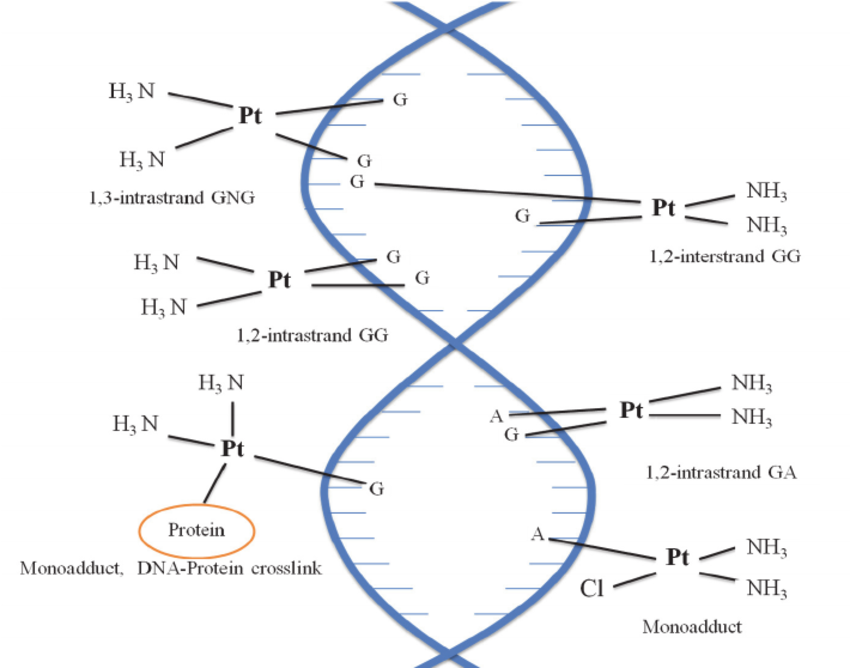
\includegraphics[width=0.5\textwidth]{Theory/cisplatin_DNA.png}
    \caption{A DNA Repair Protein BRCA1 as a Potentially Molecular Target for the Anticancer Platinum Drug Cisplatin - Scientific Figure on ResearchGate. Available from: https://www.researchgate.net/figure/Common-cisplatin-DNA-adducts-and-functions-For-instance-the-platination-of-human-serum_fig2_221919257 [accessed 12 Apr, 2020]. }
    \label{fig:cisplatin_DNA}
\end{figure}
Pt-poisoning 


\section{Radioactive decay law and Gamma-ray spectroscopy}
Gamma-ray spectroscopy is a method to identify and obtain information about radioactive nuclei present in a detector. As beta and alpha decay can result in an excited daughter product, the spectrum in fact shows the de-excitation of the daugher product. Since we know that these gamma-lines are transitions which happens right after a beta or alpha decay (or isomer transition), we identify the parent with gamma-ray spectroscopy. A detector has channels in which counts are regiserted. These channels are ... similar to the gamma-ray energy. Thus a spectrum has channels (which increases in energy) along the x-axis and and counts along the y-axis. If a detector registers many counts, it means that the state is highly populated, and the intensity of the gamma is strong (Krane, p. 351). 

\subsection{Radioactive decay law}

From here based on Krane chapter 6 \footnote{https://faculty.kfupm.edu.sa/phys/aanaqvi/Krane-Ch-6.pdf}

The activity of a nucleus is defined as the number of decayed nuclei per unit time of a radioactive product, which is equal to the radioactive decay rate 

\begin{equation} \label{eq:activity_decayrate}
   A =  \frac{dN}{dt}=-\lambda N
\end{equation}

where N is the number of nuclei, t is the time and $\lambda$ is the decay constant. Solving equation \ref{eq:activity_decayrate} gives number of decayed products at time t
\begin{equation} \label{eq:N(t)}
    N(t) = N_0 e^{-\lambda t}
\end{equation}

\noindent 
Since $N\propto$A, the relations $\frac{N_0}{A_0}=\frac{N(t)}{A(t)}$ are valid, and we can rewrite the equation \ref{eq:N(t)} to

\begin{equation} \label{eq:activity_decaylaw}
    A(t) = A_0 e^{-\lambda t}
\end{equation}


This accounts for single nucleus decaying into a daughter product, without anything first decaying into the parent nucleus. However it is common that a radioactive nucleus decays into another radioactive nucleus. Hence the daughter activity will increase due to feeding from the parent.
%The number of decayed nuclei N of nucleus i with a n-decay chain is then
%\begin{equation}
%    dN_i = \lambda_{i-n}N_{i-n}dt - ... -\lambda_{i-1}N_{i-1}dt - \lambda_iN_idt
%\end{equation}
For multiple decay, Bateman equation is used describing the activity in nucleus n of the decay chain \textcolor{red}{(Voyles2018, which article??)}

\begin{equation} \label{eq:ndecay_chains}
    A_n = \lambda_n \sum_{i=1}^n \Big[ \Big( A_{i,0}\prod^{n-1}_{j=i}\lambda_j \Big)\cdot \Big( \sum_{j=i}^n \frac{e^{-\lambda_j t}}{\prod_{i\neq j}^n (\lambda_i - \lambda_j)} \Big) \Big]
\end{equation}

where $A_n$ is the activity of nuclei n in the decay chain, with the corresponding decay constant $\lambda_n$. The equation sums over all nuclei in the decay chain. $A_{i,0}$ is the initial activity of nucleus i, and j is the nucleus which is feeding into nucleus i. 

\noindent 
If a target of stable nuclei is assumed, which is exposed to a particle beam which induces various nuclear reactions, the constant rate of production of a specific reaction is dependent on the number of target nuclei, the current of flux of the particle beam and the reaction cross section

\begin{equation}
    R = N_T \Phi \sigma
\end{equation}

\noindent 
where R is the production rate, $N_T$ is the number of target nuclei, $\Phi$ is the beam current or flux and $\sigma$ is the reaction cross section. In the assumption of the production rate being a constant value, the number of transformed target nuclei is small in comparison to the total number during the irradiation time. The number of produced nuclei from a specific reaction per unit time is thus thus the produced nuclei minus the decayed nuclei (activity)
\begin{equation}
    dN = Rdt - \lambda N dt
\end{equation}

which has the solution

\begin{equation}
    N(t) = \frac{R}{\lambda}(1-e^{-\lambda t})
\end{equation}

From equation \ref{eq:activity_decayrate}, the total activity produced during irradiation time t is thus 

\begin{equation} 
    A(t) = R(1-e^{-\lambda t}) = N_T \Phi \sigma (1-e^{-\lambda t})
\end{equation}

At the end of beam, the activity is denoted as $A_0$, and t is the irradiation time:
\begin{equation} \label{eq:activity_eob}
    A_0 = N_T \Phi \sigma (1-e^{-\lambda \Delta t_\text{irr}})
\end{equation}

\noindent 
When a target is irradiated, the activity of the product nucleus will increase until secular equilibrium is achieved, which is when the product rate and decay rate are constant. Hence it is not necessary to irradiate a target for more than 2-3 half lives.\\

\noindent 
If a spectrum is counted at a delay time $\Delta t_d$ after end of beam with a counting time $\Delta t_c$  the total number of decayed products are 

\begin{equation}
    N_D = \int_{\Delta t_d}^{\Delta t_d + \Delta t_c} A(t) dt
\end{equation}

Using equation \ref{eq:activity_decaylaw} for A(t), the solution to the above equation is 
\begin{equation} \label{eq:numb_of_decayed}
    N_D= \frac{A_0}{\lambda}e^{-\lambda \Delta t_d}(1-e^{-\lambda \Delta t_c})
\end{equation}

which again is equal to
\begin{equation}
    N_D = \frac{A(t)}{\lambda} (1-e^{-\lambda \Delta t_c})
\end{equation}

We can only know the number of decayed products which are detected. This is dependent on the efficiency of the detector, the intensity of the gamma-rays and the true number of decayed products

\begin{equation}\label{eq:Ngamma}
    N_C  = N_D \epsilon I_\gamma
\end{equation}

where $N_C$ is the number of observed/counted gamma-rays, $\epsilon$ is the efficiency of the detector and $I_\gamma$ is the gamma-ray intensity.\\ 

\noindent
Thus, we can obtain an expression for $A(t)$ after a delay time: 

\begin{equation} \label{eq:Final_Expression_A}
    A(t) = \frac{N_C \lambda}{\epsilon I_\gamma (1-e^{-\lambda \Delta t_c})}
\end{equation}

\noindent 
Again using \ref{eq:activity_decaylaw} for A(t), the above expression can be rewritten using $A_0$ and the delay time $\Delta t_d$

\begin{equation} \label{eq:Final_Expression_A0}
    A_0 = \frac{N_C \lambda }{\epsilon I_\gamma (1-e^{-\lambda \Delta t_c})e^{-\lambda \Delta t_d}}
\end{equation}
\begin{comment}
Combining equation \ref{eq:activity_eob} and \ref{eq:numb_of_decayed}, total number of decayed products is

\begin{equation} \label{eq:finalN_D}
    N_D= \frac{N_T \Phi \sigma}{\lambda}(1-e^{-\lambda \Delta t_\text{irr}})\cdot e^{-\lambda \Delta t_d}\cdot (1-e^{-\lambda \Delta t_c})
\end{equation}

Combining equation \ref{eq:Ngamma} and \ref{eq:finalN_D}, we get the following expression 

\begin{equation}
    \frac{\epsilon I_\gamma}{N_C}=\frac{N_T \Phi \sigma}{\lambda}(1-e^{-\lambda \Delta t_\text{irr}})\cdot e^{-\lambda \Delta t_d}\cdot (1-e^{-\lambda \Delta t_c})
\end{equation}

From here, $A_0$ is the following equation \ref{eq:activity_eob}

\begin{equation}
    A_0 = \frac{\epsilon I_\gamma \lambda}{N_C}\cdot e^{-\lambda \Delta t_d}\cdot  (1-e^{-\lambda \Delta t_c})
\end{equation}





%\begin{equation}
%    \sigma = \frac{A_0 }{N_T \Phi (1-e^{-\lamda \Delta t_\text{irr}})}
%\end{equation}

\begin{equation}
 \Phi = \frac{A_0 }{N_T \sigma (1-e^{-\lamda \Delta t_\text{irr}})}    
\end{equation}


\end{comment}

%In a detector, we can only know the number of decayed products from which are registered. Whether the detector detects or not is dependent on efficiency of detector, the intensity of the gamma-rays and the true number of decayed products

%\begin{equation}\label{eq:Ngamma}
%    N_\gamma  = N_D \epsilon I_\gamma
%\end{equation}

%where $N_\gamma$ is the number of observed gamma-rays, $\epsilon$ is the efficiency of the detector and $I_\gamma$ is the gamma-ray intensity. Combining equation \ref{eq:finalN_D} and \ref{eq:Ngamma}, the get the following expression 

%\begin{equation}
%    \frac{\epsilon I_\gamma}{N_\gamma}=\frac{N_T \Phi \sigma}{\lambda}(1-e^{-\lambda \Delta t_\text{irr}})\cdot e^{-\lambda \Delta t_d}\cdot (1-e^{-\lambda \Delta t_c})
%\end{equation}



\subsection{High purity Germanium detector}
High purity Germanium detector is a type of semiconductor, which is a material where the energy required to remove an electron from the valence band (in the outer atomic shell) to the conduction band is small. The germanium atom has atomic number 32, and 4 valence electrons in the outer p4 shell (need citation?). The atoms in the detector are bound through covalent bonds in a crystal structure. The main mechanism of a semiconductor is creation of electron-hole pairs after energy deposition of an ionizing particle in the crystal. If an electron is excited to the conduction band, a hole is left. This hole can move as a neighboring electron fills this spot, and it can cause a chain reaction, and the hole will move in the crystal. Both the electron in the conduction band and the  and the hole in the valence band contributes to an electric current. Under influence of an electricfield, the electron-hole pairs will be collected and we can measure the incident as a count. The major
advantage with semiconductor detector is that the average energy to create an electron-hole pair is
very low, which results in a superior energy resolution in comparison to other detectors like gas and
scintillation detectors. High energy resolution advantageous in gamma-ray spectroscopy which makes
it possible to separate to gamma-ray peaks within less than a keV. At room temperature, thermal
energy can excite the electron from the valence to the conduction band and cause noise in spectra.
Therefor, Germanium detectors are operated at 0 Kelvin. Write about recombination and trapping,
noise, np semiconductor junction, depletion depth?? (Techniques for Nuclear and Particle Physics Experiments, William R. Leo, p. 215-216). 


%\subsection{Obtaining a gamma-rey spectrum}
Ideally, for all gamma-rays with the same energy, should be detected in the same channel giving a step function. However, realistically, the resolution of a detector is not that good, and instead of seeing a delta peak, the peak is typically gaussiam shape with a finite width. The full width half maximum $\Delta E$ of the peak tells us how well the relative resolution at gamma-energy E,
\begin{equation}
    \text{resolution} = \frac{\Delta E}{E}
\end{equation}

The energy resolution is important, as it tells us how well it can distinguish two close lying peaks from each other (Techniques of Nuclear and particle Physics.. , p. 117).  The resolution of a germanium detector very good (0.1\% for a 1 MeV gamma-ray) in comparison to for instance NaI detector (8-9\% for a 1 MeV gamma-ray) (Techniques of Nuclear and particle Physics.. , p. 117). \textcolor{red}{explain why, prob in semiconductor chapter!} \\


The peak it self is not directly gaussian. Ionizing radiation statistics is based upon Poisson statistics, where  and the probability of observing N events is a discrete value

\begin{equation}
    P(N) = \frac{\mu^N e^{-\mu}}{N!}
\end{equation}

where $\mu$ is the mean value. This distribution counts when the probabiliy is a small (eg decay prob?) value and that the total number of trials are large (number of decays) (Techniques of Nuclear and particle Physics.. , p. 85).  For poisson distribution, the average is equal to the variance; $\sigma^2=\mu$. From there, the standard deviation ($\sigma$) is thus equal to the squareroot of the average. 

The distribution is not symmetric, but as $\mu$ increases in value, the peak approxes a gaussian shape. The total number of counts is the area of the peak. The total peak is a Guassian assumption but with an exponential skew towards kiw E caused by incomplete charge collection, abd a step function for taking compton backgroun into account. 

In calculation of the peak area, there are two uncertainties of relevance, the relative statistical uncertainty in the counting from the Poisson statistics, 
\begin{equation}
\sigma N_i = \sqrt{N_i}
\end{equation}

If numb of counts $N_i =10000$, the relative uncertainty ($\frac{\sigma N_i }{N_i}= \frac{1}{{sqrt{N_i}}}$=1\%). Therefor we say that a good number of counts is 10000 or more to reduce the statistical uncertainty. The other is systematic in the detector, and can for instance be due to a process called annealing, which is heat damage to the detector. Can fix by taking a blanket of resistor wrap crystal in, rise to high temp, let it sit and slowly deheat to room temp, traps will defuse and detector is repaired (this is notes from Andrew).

Also write about deadtime! 
\subsection{Gamma-ray spectrum}

Spectrum: consists of photopeaks, a compton continuum, compton edge, backscatter peak, single exscape double escape. In cases where positrons exist, chances of having a broad fat 511 keV peak. 

Germanium detecors, highest resolution for gamma-rays, from frew keV to 10 MeV. The peak to Compton ratio is much greater due to the higher photoelectric cross section of Germnaium . The largets challenges are with signal to noise ratio, it is important to shield very well to minimze background radiation (Techniques for Nuclear and particle..... William R. Leo, p. 241). \\ \\

\noindent 
here from another citation: "Practical Gamma-ray Spectroscopy". Gordon R. Gilmore. Nuclear Training Services Ltd Warrington UK. \textcolor{red}{(can be find under articles in masterthesis). This book can also be used in particle interaction in matter check!!}
In a detector, the particles interacts as the photons described in particle interaction, via photoelectric, compton scattering and pair production. Photoelectric absorption where the photon is completely absorbed by atomic electron is desired because all of the energy is deposited within the detector. For a compton scattering event, if the resulting photon's energy is also deposited in the detector (for a large detector), then the total energy would add up. Same for pair production. The photon must interact in the detector volume, and the resulting electron and positron energy is deposited in the detector volume. However when the positron slows down, it annihilates with one atomic electron, releasing two 511 keV photons. If both annihilation photons's energy is deposited in the detector volume this will also contribute to a full width peak. If one 511 photon escape and the other is deposited, there will be a peak at $E_\gamma-511$ keV, and if both peaks escape, there will a double escape peak at $E_\gamma-1022$ keV. The "degree of incomplete absorption" depends upon the size of the detector and the gamma-ray energy. As previously discussed photoelectic effect dominates at low energies, and the less compton scattering and of course pair production (for E gamma higher than the threshold.). The detector size also matters because the larger the more room for the photon to scatter in and lose energy before escaping. (p. 32) \\

The total spectrum can be seen on p. 33 in the book. Pile-up is done because of random summing, determined by the statistical probability of two gamma-rays being detected at the same time and therefor on the sample count rate. 

Interaction with detector shielding: Photoelectric effect can be followed by emission of characteristic X-ray of the absorbing medium. X ray can escape the shielding and be deteced by the detector. Compton scattering: most gamma rays are scattered through the a large angle by the shielding, BACKSCATTERED. Whatever the initial enervy  was (if scattered by more than 120 degrees) are within 200-300 keV. Peak appears as broad. Pair production: annihilation peak (511 peak) caused by the escape of one of the 511 keV photons from the shielding following annihilation of the pair production positron. Analogous to the single and double escape mechanisms within the detector but only on 511 keV photons can ever be detected since they are emitted in the opposit direction. So in order to have a 511 peak, energy of gamma ray must be more than 1022 keV. (p. 34-35).

The 511 peak can also be expected when postron emitters are present since beta + particle interacts with electron.  

Since Compton scattering can be in a spectrum of energies, the gives rise to a Compton continuum, before the gamma-ray escapes the detector. 


The shape of the peak: The peak is a histogram that approximate a Gauss curve (p. 186). Peak searching (SAMPO) using first and second order derivatives to search for peaks (p.185)
Due to incomplete charge collection (that electron or holes are not collected) no matter how caused moves counts from the centre of the Gaussian distribution to lower channels, creating a low energy tale to the peak (p.135).  

\textcolor{red}{Include a picture of peak shape and gamma-ray spectrum!! from the same book}


\section{General nuclear reaction theory}

\textcolor{red}{paragraph based on special curriculum}
Medical radionuclides can be produced directly using charge particle (cyclotron) or neutron beams (reactors), or indirectly using radionuclide generators or fission (reactor). Medical radionuclides are typically produced in reactors, cyclotrons or by a longer lived-parent decaying into a short-lived daughter in a radionuclide generator system. In general, the production should be cheap, available. Today many radionuclides are only produced in reactors, which is the main source of neutrons, and with reactors aging (Chai Hong Yeong, Mu hua Cheng, and Kwan Hoong Ng. Therapeutic radionuclides in nuclear medicine: Current and future prospects. Journal of Zhejiang University: Science B,
15(10):845–863, 2014.), we need alternative routes to produce critical radionuclides. Cyclotrons have many benefits, like size so that it can be produced directly at the site of usage. One of the major disadvantages is that there is a need to enriched targets to get the desired reaction, and those can be very expensive. Along with high beam intensity the melting of the target can give challenges, so target cooling technqueis need to be there.    

In order to create isotopes, nuclear reactions need to occur. There are many different production routes available for a single radionuclide, which is dependent on multiple factors such as choice of target, incident particle-beam and beam energy. To each reaction route, there is an corresponding excitation function which tells us how probable the reaction channel is at various energies. The nuclear reaction data is very important for the optimization of the product, achieving minimal level of isotopic impurities and maximum yield (S M Qaim, R Capote, and F Tarkanyi. Nuclear Data for the Production of Therapeutic Radionuclides.
Trs 473, (473):395, 2011., p. 3). \\

Isotopic purity is important as it is impossible to separate isotopes of the same element (Syed M. Qaim. Nuclear data for production and medical application of radionuclides:
Present status and future needs. Nuclear Medicine and Biology, 44:31–49, jan 2017.). An undesired radionuclided can lead to undesired dose to healthy tissue, and a non-radioactive nuclide may lead to  poisoning (if large amounts injected), but it will not have any therapautic effect. This is especially important when working with poisoneos elements such as platinum. The only option to minimize isotopic impurities is to choose an appropritate energy window. 


Using charged particles instead of neutrons allows for measurement at multiple energies as the particle energy degrades in the foils. The neutron energy is not degraded in the same way, due to electric neutrality, thus can only give cross section at one single energy. 







\subsection{Nuclear reactions and reaction cross sections}

A nuclear reaction occurs when a collision between two nuclei or a nucleus and a subatomic particle takes place. Collision between an accelerated subatomic particle or small nucleus and target nuclei is common in isotope production. A nuclear reaction is denoted as
\begin{equation}
    X(a,b)Y
\end{equation}

\noindent where X is the target, a is the incoming projectile, b is the outgoing decay channel and Y is the product of the nuclear reaction (Krane, chapter 11.1). There are multiple processes which can occur, radiative capture is the process where a particle is captured and a $\gamma$-ray is emitted in a (x,$\gamma$) process. If the incoming and outgoing particle is the same, it is a scattering process, where elastic scattering leaves the target nucleus in the energy same state, and inelastic if the target nucleus is in an excited state. In these type of experiments however, we are interested in emission of particles to create products in which we can measure the reaction cross section. \\

In a nuclear reaction, the total energy and linear momentum, proton and neutron number, angular momentum and parity are conserved quantities (assuming no meson formation) (Krane, p.380). In the low energy-region in which isotope production typically takes place (\textcolor{red}{<80 MeV}?), compound nucleus reactions take place, where an incoming particle and target nucleus merges by sharing the kinetic energy on all nucleons, and particle emission takes place to reduce the excess energy. \textcolor{blue}{\footnote{blue text:https://web-docs.gsi.de/~wolle/TELEKOLLEG/KERN/LECTURE/Fraser/L24.pdf }Involves nucleon nucleon interactions, lead to a complete therman equlibrium inside the CN. Releases energy by emission of neutrons, protons, alpha particles and gamma rays. A consequence of equilibrium is that the decay of CN should not depend on the way it was formed. "forgets" in all the collisions. Consequently, the decay of the compound nucleus depends only on the mass and atomic numbers, excitation energy and angular momentum.} The contrary are direct reactions, where an incoming particle interacts (over such a short time period) so that the incoming particle only interacts with one single nucleon, typically on the surface of the target nucleus. \textcolor{blue}{Angular distributions of direct reaction products are sensitive to the momentum transfer and parity change during the reactions. Thus based on the selection rules from angular momentum and parity conversion the angular distribution measurements in direct reactions yield spin and parities of states populated in the exit channel}.  \\

%A nuclear reaction in the energy ranges of isotope production via the Compound nucleus conserves quantities such as mass-energy, linear momentum, the total number of nucleons, angular momentum and parity \textcolor{red}{cite, Krane?}. 

\noindent 
The cross section for a reaction can be divided into the cross section of the formation of the compound nucleus via interaction with the incoming projectile a, and the probability that the compound nucleus decay by decay channel b. The total reaction cross section is thus the sum of all the different reaction channels (Handbook of nuclear chemistry, p. 157 (nuclear reactions)), 
\begin{equation}
    \sigma = \sum_b \sigma(a,b)
\end{equation}
where b can be multiple particles. The general equation which is used to calculate cross sections in this experiment (solving equation \ref{eq:Final_Expression_A0}) is the following equation 

\begin{equation}
    \sigma(E) = \frac{A_0 \cdot t_\text{irr}}{N_T \cdot \Phi(E)(1-e^{-\lambda t_\text{irr}})}
\end{equation}
\noindent where $A_0$ is the end of beam activity of the resulting product nucleus (Y), $t_\text{irr}$ is the irradiation time, $N_T$ is the number of target nuclei (X), $\Phi(E)$ is the projectile flux or current (a), and $\lambda$ is the decay constant of the product nucleus. \\ 


\noindent The compound nucleus model (Bohr, 1936) is a model which describes the formation of a compound nucleus by absorption of an incoming projectile by a nucleus close enough to interact with the strong nuclear force, and the decay of the compound nucleus. The kinetic energy shared between the incoming projectile and the nucleon which was struck leads to multiple collisions with other nucleons and rapid exchange of energy. The energy is distributed throughout the nucleus, leaving the original nucleus in an highly excited state. The average energy per nucleon is not sufficient to overcome the binding energy of the nucleus, but due to the statistical distribution in energies there is a probability that one or more nucleons may get sufficient energy to escape the nuclear potential (Krane, chapter 11.10, p. 416). This is decay of the compound nucleus, and this will lower the excitation energy. We can include the formation of the compound nucleus in the nuclear reaction as \begin{equation}
    X + a \rightarrow C^* \rightarrow Y + b
\end{equation} where $C^*$ is the excited compound nucleus (Krane, chapter 11.10, p. 416)  \\

\noindent For each possible decay channel of the compound nucleus, there is an associated probability or cross section, which is dependent on the energy of the incoming projectile. A function which evaluates the various cross sections at different energies is called an excitation function. In figure \ref{fig:pt_reactionchannels}, the excitation function of the reactions channels for the platinum isotopes $^{188, 189, 191,193m}$Pt resulting from deuterons on natural iridium is plotted (using TENDL nuclear reaction code \textcolor{red}{cite}). Natural iridium consists of two stable isotopes, $^{191}$Ir (37.3\% abundance) and $^{193}$Ir (62.7\% abundance). $^{193m}$Pt can only be produced from $^{193}$Ir, ejecting 2 neutrons in the process, which can be denoted as $^{193}$Ir(d,2n)$^{193m}$Pt ($^{193}$Pt is the compound nucleus formation of deuteron on $^{191}$Ir, which has a low production cross section). The other platinum isotopes can be produced as $^{191}$Ir(d,2n)$^{191}$Pt or $^{193}$Ir(d,4n)$^{191}$Pt, $^{191}$Ir(d,4n)$^{189}$Pt or $^{193}$Ir(d,6n)$^{189}$Pt and $^{191}$Ir(d,5n)$^{188}$Pt or $^{193}$Ir(d,7n)$^{188}$Pt. For each reaction route possible, there is a local maximum for the specific route, hence, $^{193m}$Pt has only one maxima, and the other platinum isotopes has two. The desired particle emission is energy dependent, and the higher energy provided to the compound nucleus, the probability that more particles will be emitted is higher (Krane, chapter 11.10, p. 419). When a specific isotope is desired, the excitation function can tell us which energy window that maximizes the production and most importantly minimizes particularly other isotopes of the same element, due to the difficulty of separating same chemical elements. \\

\begin{figure}
    \centering
    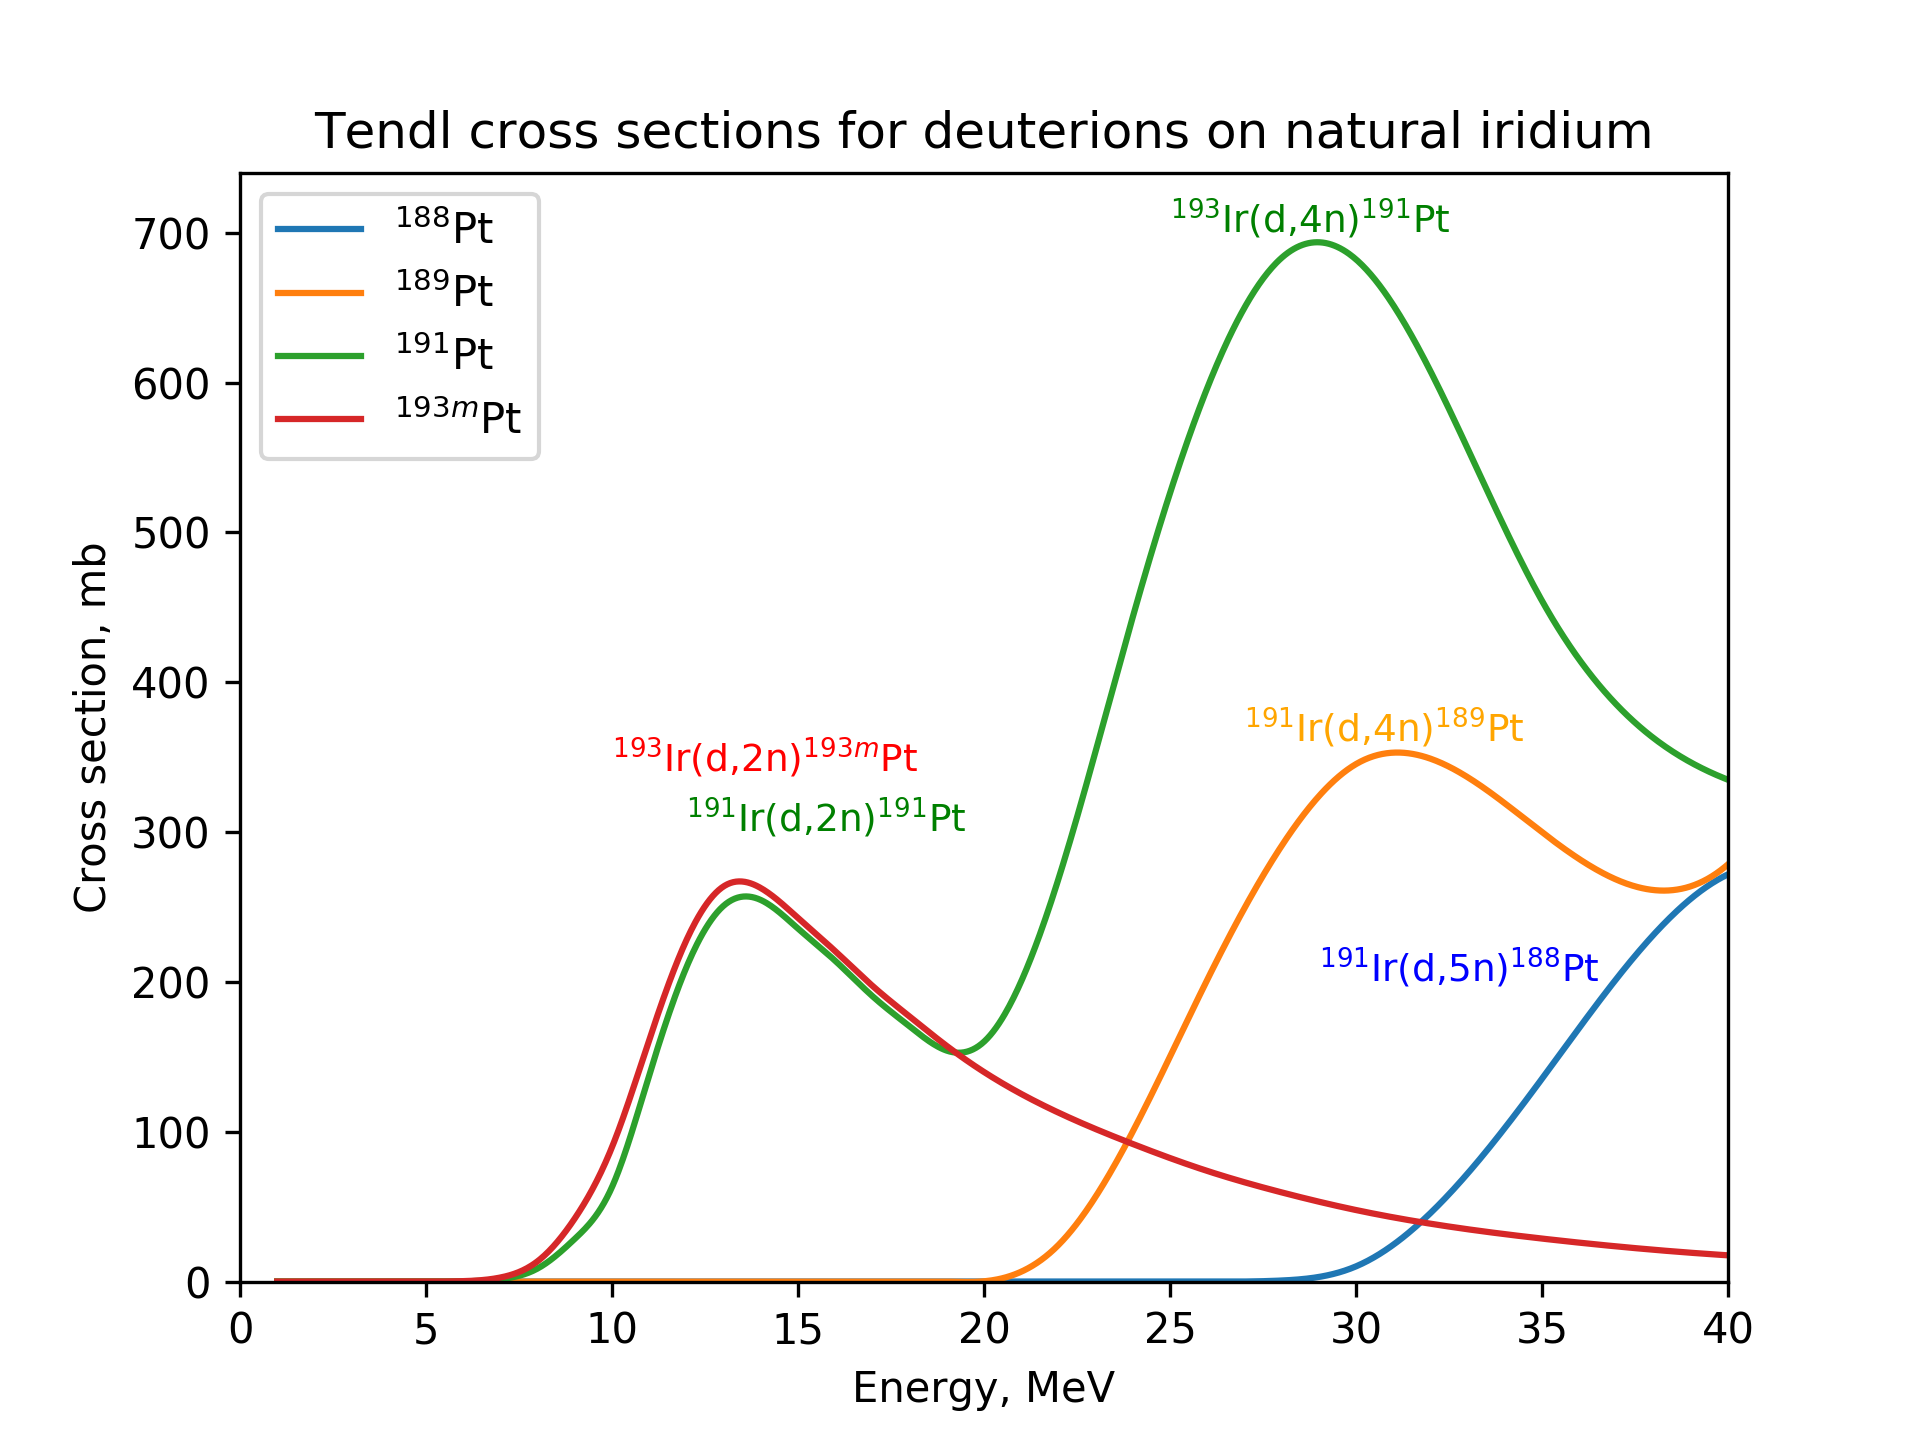
\includegraphics{Theory/reactionchannels_pt.png}
    \caption{Reaction cross sections provided by Tendl for the reactions $^\text{nat}$Ir(d,x)$^{188,189,191,193m}$Pt}
    \label{fig:pt_reactionchannels}
\end{figure}
\begin{comment}
\begin{figure}
    \centering
    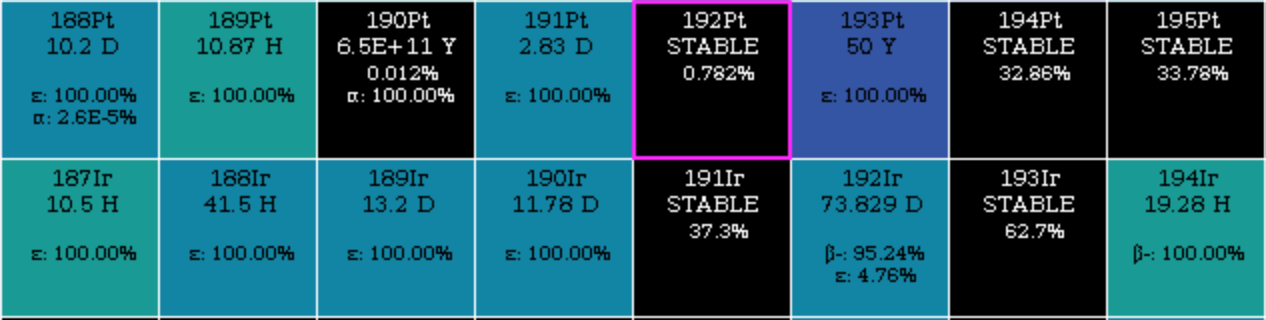
\includegraphics[width=12cm]{Ir(d)Pt.png}
    \caption{Nuclear chart for the platinum isotopes which can be produced from natural iridium }
    \label{fig:chart_irpt}
\end{figure}
\end{comment}


%\noindent A nuclear reaction
%The nucleus is built up on protons and neutrons, and these are bound through the strong nuclear force. 
\subsection{Constraints in nuclear reactions}
%\subsection{Energetic factors in nuclear reactions}

%\subsection{Dependence of }

%\noindent The binding energy depends on multiple parameters, which are based upon two models, the shell model and the liquid drop model (Krane, chapter 3.3, p. 68). The binding energy thus depends on the volume, which is constant throughout the nucleus, hence a volumeterm $a_V\cdot A$, a the surface of the nucleus which needs to be taken into account, since the nucleons on the surface is less tightly bound, $a_s\cdot A^{2/3}$. 
The potential energy of a nucleus is the sum of the attractive well from the strong nuclear force and the repulsive Coulomb barrier which acts repulsive between charged particles and the nucleus, acting long range (p. 152, Handbook of nuclear chemistry). The radius of the potential well is up to a few femtometer. For a positively charged particle induced nuclear reaction, the energy of the particle should exceed the barrier, or there will be an elastic scatter. However, there is a chance of tunneling, which drops with a factor 1/r where r is the distance from the center of the nucleus (Handbook of Nuclear Chemistry, chapter 3 - Nuclear Reactions, section, 3.2.3). The barrier also constraints the emission of particles for a decay channel of the compound nucleus, as the energy for an outgoing decay channel of positive particles must exceed the barrier. There is also a centrifugal barrier, which is dependent on the orbital angular momentum of the the nucleus.  However, this barrier is more important in 

The height of the Coulomb barrier is dependent on the radius and charge of the incoming or outgoing particle a and the target nucleus b.

\begin{equation}
    U_\text{Coulomb} = \frac{1}{4\pi \epsilon_0} \frac{e^2Z_a Z_b}{r_a + r_b}
\end{equation}

In addition, there is a centrifugal barrier, which can constraint some of the incoming particle energy in rotational energy, \textcolor{red}{which depends on the angular momentum of the incoming particle and and the nucleus???} (handbook of nuclear chemistry p. 155.)

\begin{equation}
    U_\text{centrifugal} = \frac{\hbar \ell (\ell+1)}{r^2}
\end{equation}

The sum of the barriers are the total barrier but the Coulomb barrier is the most important. 

%The orbital angular momentum is dependent on the mass and energy of the particle, but also the impact parameter of the reaction, which is the "distance" between the projectile and the nucleus

%\begin{equation}
%    \ell\hbar = (mv)b, \quad b\leq r_a + r_X
%\end{equation}

%\noindent where $r_a$ and $r_X$ are the radii of projectile and target nucleus. If $\ell=0$, the impact parameter is zero. If $\ell\neq 0$, then some of the energy of the projectile will go to rotational energy of the nucleus (Handbook of Nuclear Chemistry, chapter 3 - Nuclear Reactions, section, 3.2.4). The probability of this drops with $1/r^2$, and if the impact parameter is large, this will constraint some of the energy that would have gone to the nuclear reaction. Figure \ref{fig:sumOfPotentials} shows an overview of the various potentials; centrifugal barrier, Coulomb barrier and nuclear potential. The figure is for $^{58}$Zn, but the figure is only an example. \textcolor{red}{maybe make figure self?}. 


\begin{figure}
    \centering
    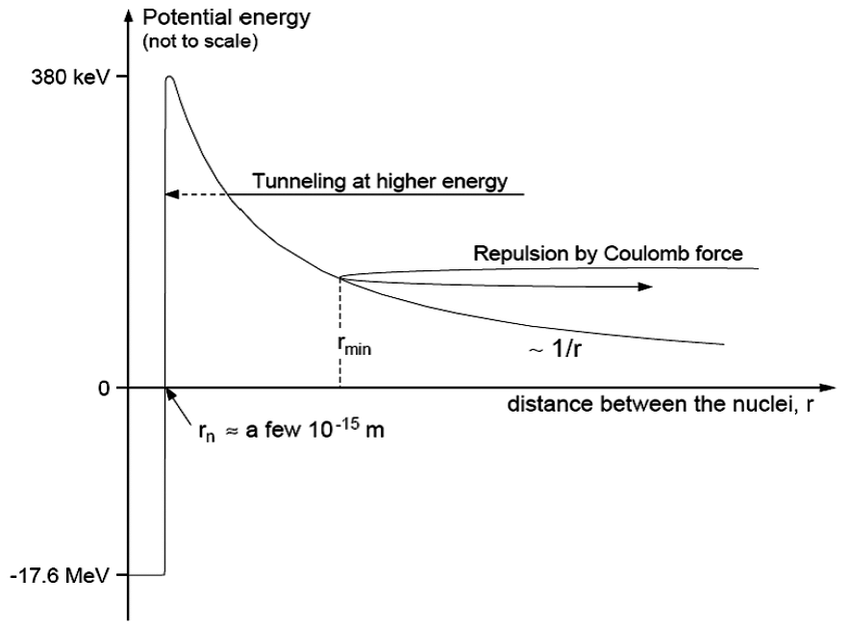
\includegraphics[width=8cm]{Theory/Coulomb_barr.png}
    \caption{ }
    \label{fig:Coulomb_barrier}
\end{figure}



\begin{comment}
\noindent The separation energy is the energy required to remove a particle from the nucleus. That is the difference in the binding energy for the two nuclei. The neutron separation energy is 
\begin{equation}
    S_n = B(^A_z X_n)-B(^{A-1}_z X_{n-1}) = c^2(m(X^{A-1}_zX_n)-()
\end{equation}\\ 
\end{comment}

\noindent In a nuclear reaction, the mass-energy is conserved, which is denoted as the Q-value. The reaction Q-value is the difference is masses between before and after the nuclear reaction occurred (Krane, chapter 11.2). It is defined as 

\begin{equation} \label{eq:Q_value}
    Q = (m_i - m_f)c^2 = (m_X + m_a - m_Y - m_b)c^2
\end{equation}

\noindent where $m_i$ is the initial mass, $m_f$ is the final mass and c is the speed of light. If $Q>0$, then the reaction is exoergic, which means that energy is released in the reaction. There is no threshold energy of the projectile required for the reaction to occur, if only the projectile is present the reaction can occur. If $Q<0$, then the reaction is endoergic, which means that the kinetic energy of the incoming projectile is converted into nuclear mass or binding energy. For endoergic reactions to occur, there is a minimum threshold energy of the projectile in order for the reaction to happen, which is defined as (Krane, 11.2, p. 382)

\begin{equation} \label{eq:reaction_threshold}
    E_\text{threshold} = (-Q) \cdot \frac{m_Y +m_b}{m_Y + m_b -m_a}
\end{equation}


\noindent The energy threshold thus depend on the Q-value, the Coulomb barrier for charged particles, and the centrifugal barrier if angular momentum $\ell\neq 0$. The parity though depend, even numbers of $\ell$ mix with even, and odd with odd (Handbook of Nuclear Chemistry, chapter 3Nuclear Reactions, section, 3.2.3). This gives an indication on when a reaction can energetically occur, but does not tell us how probable the reaction is. %Equation \ref{eq:reaction_threshold} indicates that a higher mass for the particle in the outgoing channel $m_b$, will lower the energy threshold.\\ 

%The nuclear binding energy is a number which tells us how tightly bound the nucleus is, and how much energy is required to separate nucleons from the nucleus. The nuclear binding energy is related to the mass of the nucleus, through the famous equation   E=mc^2

The binding energy is the mass-difference between the nucleus as a whole, and the number of protons and neutrons added
\begin{equation} \label{eq:Binding_energy1}
    B = c^2(z\cdot m_p + n \cdot m_n - m_N)
\end{equation}
\noindent where z is the number of protons, n is the number of neutrons, $m_p$ is the proton mass, $m_n$ is the neutron mass, $M_N$ is the mass of of the nuclide, which is the number of nucleons A minus the number of electrons, $M_P = m_A - z\cdot m_e$ (the electronic binding energy per electron is excluded). From Krane's derivation of the nuclear binding energy (Krane, chapter 3.3, p. 65). 

From equation \ref{eq:Q_value}, the larger the mass of the outgoing decay channel, the more negative the Q-value will be. Protons (+1 charge) and neutrons (neutral) are the simplest decay channels of the compound nucleus, each carry a spin of $1/2$, with masses $m_p=938.28$ MeV/c$^2$, and $m_n=939.57$ MeV/c$^2$. Combinations like deuterons (d=1p+1n, charge +1) has a mass difference of $\Delta=$2.2 MeV/$c^2$ from realising 1 proton and 1 neutron separately, a triton (t=2n+1p, charge +1) with $\Delta=8.5$ MeV/$c^2$,  3-Helium ($^{3}$He=1n+2p, charge +2) with $\Delta=7.7$ MeV/$c^2$ and alpha-particle ($\alpha$=2n+2p, charge +2) with $\Delta=28.3$ MeV/c$^2$. Thus, Q-values are higher in value, the lighter the particle is. However, in this work, we can clearly see that protons, neutrons and alpha-particles are strongly fed decay channels, while the other don't even appear. The suggested reason for this is that due to \textcolor{red}{blablabla nuclear physics stuff, like shell structure}, protons and neutrons are favoured, but since the alpha-particle has such a large binding energy, this channel is also favoured.  

\subsection{Nuclear reaction models}

The optical model (proton/neutron, and alpha/deuteron), gamma strength function. 

\subsubsection{EMPIRE 3.2.3}
\subsubsection{CoH 3.5.3}
\subsubsection{ALICE 2017}
\subsubsection{TALYS 1.9}
\subsubsection{TENDL 2019}



%, the equal number of protons and neutrons make up $z\cdot^1H$, thus we can rewrite equation \ref{eq:Binding_energy1} to 

%\begin{equation}
%    B = z\cdot m_{^{1}H} + n\cdot m_n - m_{A}
%\end{equation}

%\noindent 
%Separation energy of a particle is the energy required to be removed from the nucleus. This is defined as the difference in binding energy between the nucleus with the particle and the nucleus without the emitted particle. Since heaavier particles such as tritrium has a lower binding energy, more energetically easy to separate. n and p require more. 



\begin{comment}

\subsection{Nuclear cross sections}

The cross section for a reaction can be divided into the cross section of the formation of the compound nucleus via interaction with the incoming projectile a, and the probability that the compound nucleus decay by decay channel b. The total reaction cross section is thus the sum of all the different reaction channels, 
\begin{equation}
    \sigma = \sum_b \sigma(a,b)
\end{equation}
where b can be multiple particles. The general equation which is used to calculate cross sections in this experiment is the following equation, which is solved from equation \ref{eq:activity_eob} (referenced to in the later parts of the paper)

\begin{equation} \label{eq:cross_section_equation}
    \sigma(E)=\frac{A_0}{N_T\Phi(E)(1-e^{-\lambda \Delta t_\text{irr}})}
\end{equation}

not, need to check if this is the correct one.. 
\begin{equation}
    \sigma(E) = \frac{A_0 \cdot t_\text{irr}}{N_T \cdot \Phi(E)(1-e^{-\lambda t_\text{irr}})}
\end{equation}
\noindent where $A_0$ is the end of beam activity of the resulting product nucleus (Y), $t_\text{irr}$ is the irradiation time, $N_T$ is the number of target nuclei (X), $\Phi(E)$ is the projectile flux (a), and $\lambda$ is the decay constant of the product nucleus. 

\newpage

Why we are interested, why is there a need for nuclear production cross sections. 



The Q-value for nuclear reactions 

Compound nucleus, what happens. 
Q value, binding energy, particle emission, probabilities (why does n, p/alpha emission require higher energy, but is more favoured than T emission if both possible.)


\subsection{Expected products from deuterions on iridium, iron, cupper and nc}

Include figure of different nuclear charts, and write about Q values, and reaction channels, which makes it more probable that we observe it (eg. when neutron, proton/alpha channels opens).





\section{From book}

In a nuclear reaction, the energy, linear momentum, the total number of protons and neutrons, angular momentum and conservation of parity is conserved. \\

The compound nucleus; the collisions are described by a model called Multistep Compound Model (Feshback, Kerman and Koonin, 1980), which is the model that reaction modeling code EMPIRE and TALYS rely on. \textcolor{red}{find out what ALICE does ???}

Products of a nuclear reaction can be anything than conserve the various variables. Mass energy conservation is the Q-value, which is the mass differene in the reactant nuclei (projectile and target in this case) and product nuclei (decay channel particles and product). Binding energy (nuclear mass energy) often denoted as $\Delta=(M_0 - Au)c^2$, where A is atomic mass number, u is atomic mass unit. Q-value can be rewritten: 
\begin{equation}
    Q = \Delta_\text{projectile} + \Delta_\text{target} - \sum \Delta_\text{products}
\end{equation}

Charged particle reactions with heavy nuclei which is the case here, can have positive or negative Q-value. If the Q-value is negative, energy is required to induce the reaction. The reaction is negative if the sum of products is less than the sum of reactants. The excitation energy of the product nucleus is the extra energy which is deposited in the product nucleus. The decay of this is often times $\gamma$-rays (?). If the excitation energy is lower than the binding energy of the nucleus?  Threshold is the minimum energy required for the incoming projectile to form a product nucleus, which is then in its ground state. 

\begin{equation}
    \text{mass-energy}: \quad \Delta_t+ \Delta_p + E_p 
\end{equation}




\section{The decay of the compound nucleus}
At the energy ranges in which this work is operating in, the nuclear reaction is caused by a fusion between the incoming projectile to create an highly excited compound nucleus. \\ 

\noindent 
The decay favoured decay channel is dependent on multiple properties such as the charge and angular momentum. The coulomb potential is defined as 

\begin{equation}
    U_{c} = K\frac{z_1 z_ 2 e^2}{A_1^{1/3} + A_2^{1/3}}
\end{equation}

where z is the the number of charges, e is the electrical charge and $A^{1/3}$ is the nuclear radius which is equal to $r=r_0 A^{1/3}$. K is a constant value. 

The centrifugal barrier (which is the amount of energy which is conserved in rotational energy) depends on the angular momentum 

\begin{equation}
    U_{s} = \frac{\hbar \ell(\ell+1)}{2\mu r^2}
\end{equation}

where $\mu$ is the reduced mass $u\cdot \frac{A_1 A_2}{A_1 + A_2}$. 


\textcolor{red}{Table \ref{tab:decaychannel_particles} might be wrong in the sense $J^\pi$. Might just be the total spin which is of interest? But since $J=l+s$, the spin will give a higher intrinsic angular momentum. Since $|I_i - I_f| \leq \ell \neq I_i+I_f$, $\ell$ can be multiple values, and the parity is thus dependent on the value here. (Krane, chapter 8.5, p. 257). The centrifugal potential is thus} 

\begin{equation}
   U_{0,s} =  \frac{\ell (\ell +1)\hbar}{2mr^2}
\end{equation}

and the Coulomb potential is

\begin{equation}
    U_{0,c} = K\frac{z_1 z_2 e^2}{A_1{1/3}+ A_2^{1/3}}
\end{equation}

The 

\begin{table}[]
    \centering
    \caption{The table shows the most common decay channels for the decay routes available in this energy region. $\Delta$ is the binding energy of the alpha particle, which can be calculated using equation \ref{eq:Binding_energy1}, where the mass of the proton is $m_p = 938.28$ MeV/c$^2$ and $m_n=939.57$ MeV/c$^2$. $\Delta$ is thus the difference in in energy-mass between the particle composed of protons and or neutrons, and a equal number of protons and neutrons independent. All parities are positive due to angular momentum $\ell=0$.  }
    \begin{tabular}{|c|c|c|c|c|}
         \hline 
         Particle & \Delta (MeV) &J^\pi & Charge \\
         \hline
         p & - & $\frac{1}{2}^+$ & +1 \\
         n & - & $\frac{1}{2}^+$ & 0 \\
         d & 2.2 & $1^+$ & +1 \\
         t & 8.5 & $\frac{1}{2}^+$ & +1 \\
         ^{3}He & 7.7 & $\frac{1}{2}^+$ & +2 \\
        \alpha & 28.3 & 0^+ & +2 \\
        \hline
    \end{tabular}
    \label{tab:decaychannel_particles}
\end{table}


\begin{table}[]
    \centering
    \begin{tabular}{|c|c|c|c|c|c|c|}
        \hline
        Target & Proton & neutron & deuterion & triton & ^{3}H & \alpha  \\
        \hline
        Fe (Z=26) & & & & & &  \\
        Ni (Z=28) & & & & & &  \\
        Cu (Z=29) & & & & & &  \\
        Ir (Z=30) & & & & & &  \\
        
    \end{tabular}
    \caption{The Coulomb barrier in MeV for each of the targets. Can be used to explain why we see what we see. }
    \label{tab:my_label}
\end{table}

The total angular momentum J is the sum of the orbital and intrinsic angular momentum (spin), thus 
\begin{equation}
    \mathbf{J} = \mathbf{\ell} + \mathbf{s} 
\end{equation}

The spin is the sum of unpaired paired protons and neutrons. The total nuclear spin is thus $I = \sum_i J_i$.  The value of the angular momentum is
\begin{equation}
    |I_i - I_f| \leq \ell \geq |I_i + I_f|
\end{equation}

Thus, 





\end{comment}